\documentclass[a4paper]{article}
\usepackage[T2A]{fontenc}
\usepackage[utf8x]{inputenc}
\usepackage[english,russian]{babel}
\usepackage{multicol}
\usepackage{fancyhdr}
\usepackage[warn]{mathtext}
\usepackage{graphicx}
\usepackage{microtype}
\usepackage{wrapfig}
\usepackage{amsmath}
\usepackage{floatflt}
\usepackage{geometry} \geometry{verbose,a4paper,tmargin=2cm,bmargin=2cm,lmargin=1.5cm,rmargin=1.5cm}
\usepackage{float}
\usepackage{amssymb}
\usepackage{caption}
\usepackage{epsfig}
\usepackage{newunicodechar}

\begin{document}

\pagestyle{fancy} 
\fancyhead[R]{Спектр $H$ и $I$}
\fancyhead[L]{Квантовая физика}
\fancyhead[C]{}
\fancyfoot[C]{ \noindent\rule{\textwidth}{0.4pt} \thepage }

\begin{titlepage}
	\centering
	\vspace{5cm}
    {\scshape\LARGE Московский физико-технический институт\par}
    

	\vspace{3cm}
	{\scshape\Large Лабораторная работа по общей физике \par}
	\vspace{1cm}
    {\huge\bfseries  2.2 и 2.3 Изучение спектров атомов водорода и молекулы йода \par}
	\vspace{1cm}
	\vfill
\begin{flushright}
	{\large выполнил студент Б04-852 группы ФЭФМ}\par
	\vspace{0.3cm}
	{\LARGE Яромир Водзяновский}
\end{flushright}

	
	\vfill
Долгопрудный, 2020
% Bottom of the page
\end{titlepage}


\section{Цель работы}
\begin{enumerate}
    \item Исследование сериальных закономерностей в оптическом спектре водорода
    \item Исследование спектра поглощения паров йода в видимой области
    \item Вычисление постоянной Ридберга для водорода по результатам измерения
    \item Вычислить энергию колебательного кванта молекулы йода и энергию диссоциации в основном и возбужденном состояниях.
\end{enumerate}

\section{В работе используются}
\begin{itemize}
    \item стеклянно-призменный монохроматор-спектрометр УМ-2
    \item Неоновая лампа
    \item ртутная лампа ПРК-4 для градуировки 
    \item водородная лампа
    \item Кювета с кристаллами йода
\end{itemize}

\section{Теоретические положения}
\subsection{Водород}
Длины волн спектральных линий водородоподобного атома описываются формулой
\begin{equation}
    \frac{1}{\lambda_{mn}} = RZ^2(\frac{1}{n^2} - \frac{1}{m^2}),
\end{equation}
где $R$ - постоянная Ридберга, а $m, n$ -  целые числа. \par
Использование постулатов Бора с учётом кулоновского взаимодействия между ядром и электроном 
позволяет легко определить возможные энергетические состояния водородоподобного атома. Если 
считать ядро неподвижным, то эти энергетические состояния определяются выражением
\begin{equation}
    E_n = -\frac{2 \pi^2 m_e e^4 Z^2}{h^2} \frac{1}{n^2}
\end{equation}


Знание энергетических состояний атома позволяет в соответствии с формулой (2) определить 
возможные частоты его излучения и объяснить наблюдаемые закономерности. \par
В данной работе изучается серия Бальмера, линии которой лежат в видимой области, и изотопический 
сдвиг между линиями водорода. Для серии Бальмера в формуле (1) $n = 2$. Величина $m$ для первых 
четырёх линий этой серии принимает значение 3, 4, 5, 6. \par

\begin{figure}[H]
    \begin{center}
    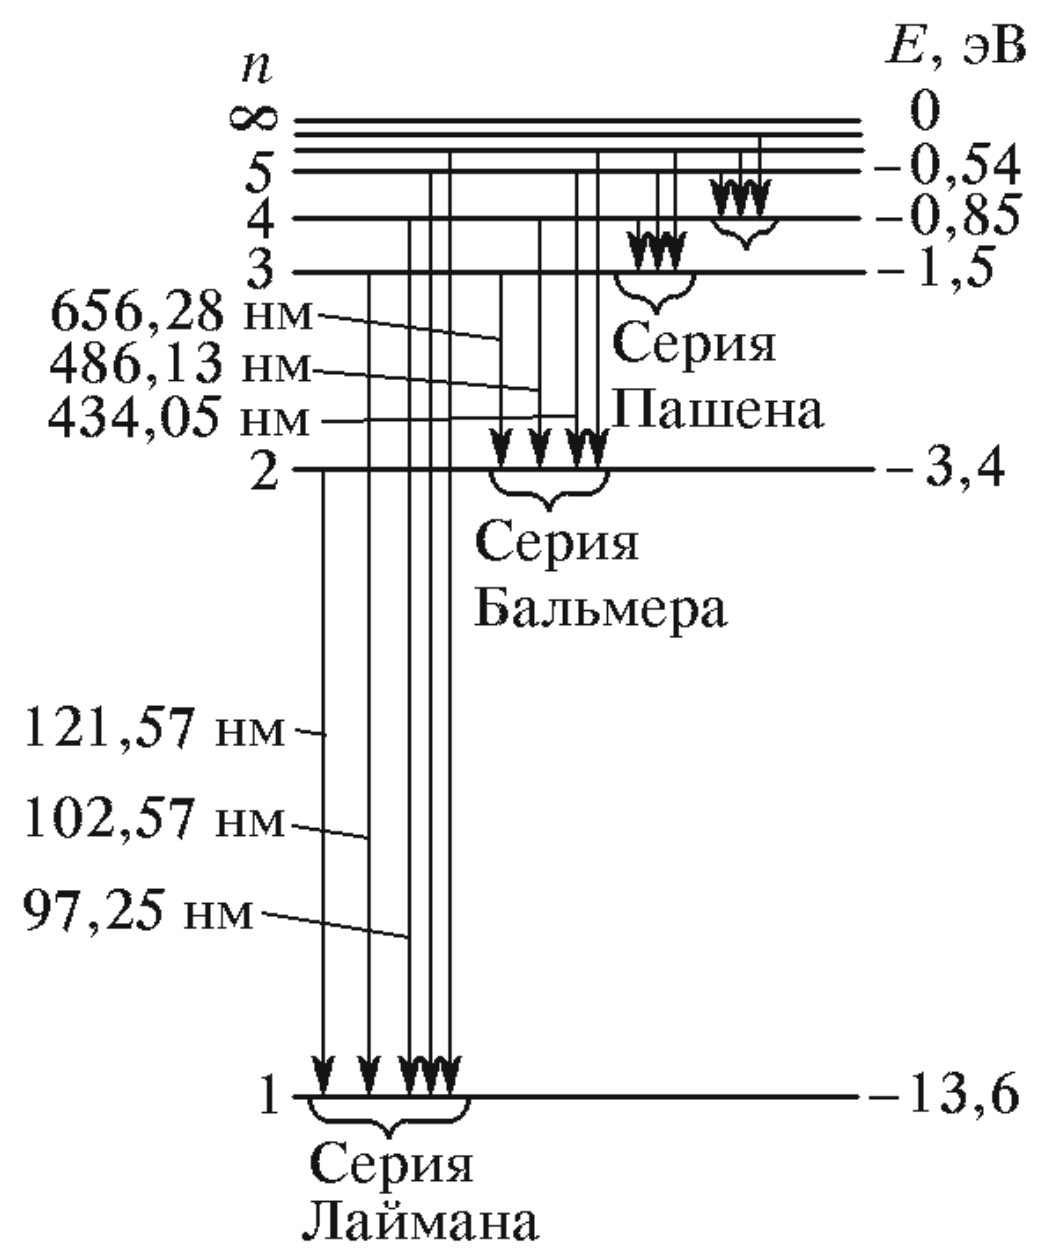
\includegraphics[scale = 0.3]{p1.png}
    \caption{}
    \label{p1}
    \end{center}
\end{figure}

Боровский радиус (радиус первой орбиты) для электрона в поле ядра с зарядом $Z$:
\begin{equation}
    r_B = \frac{\hbar^2}{Z m_e e^2}
\end{equation}
Энергия основного состояния:
\begin{equation}
    E = -\frac{m_e e^4}{2 \hbar^2}Z^2 = -R Z^2
\end{equation}
Аналогичным образом могут быть найдены энергии возбуждённых состояний. Дискретные значения 
энергии электрона в атоме получаются из того условия, что на длине орбиты, по которой движется 
электрон, должно укладываться целое число волн де Бройля. Если радиус орбиты равен $r$, то $n$-му 
состоянию электрона соответствует условие 
\begin{equation}
    2 \pi r = \lambda n (n \in \mathbb{N}) ; m_e v_n = \frac{nh}{2 \pi r}
\end{equation}

Аналогично пп. (3)-(4):
\begin{equation}
     r_B = \frac{n^2 \hbar^2}{Z m_e e^2}
\end{equation}

\begin{equation}
    E = -\frac{m_e e^4}{2 \hbar^2} \frac{1}{n^2} Z^2 = -R \frac{Z^2}{n^2}
\end{equation}

\subsection{Йод}

Молекулы обладают более багатым спектром возбужденных состояний, чем изолированные атомы:
$$E = E_{\text{эл}} + E_{\text{колеб}} + E_{\text{вращ}}$$

Соотношения соответствующих частот:
$$\omega_{\text{эл}} : \omega_{\text{колеб}}: \omega_{\text{вращ}} \approx 1 : \sqrt{
    \frac{m}{M}} : \frac{m}{M} \approx 1 : 10^{-3} : 10^{-6}
$$

Оптические переходы связаны с излучением/поглощением квантов света сопровождаются изменением вращательного
и колебательного состояний. Идет наложение колебательного спектра на электронный:

\begin{figure}[H]
    \begin{center}
    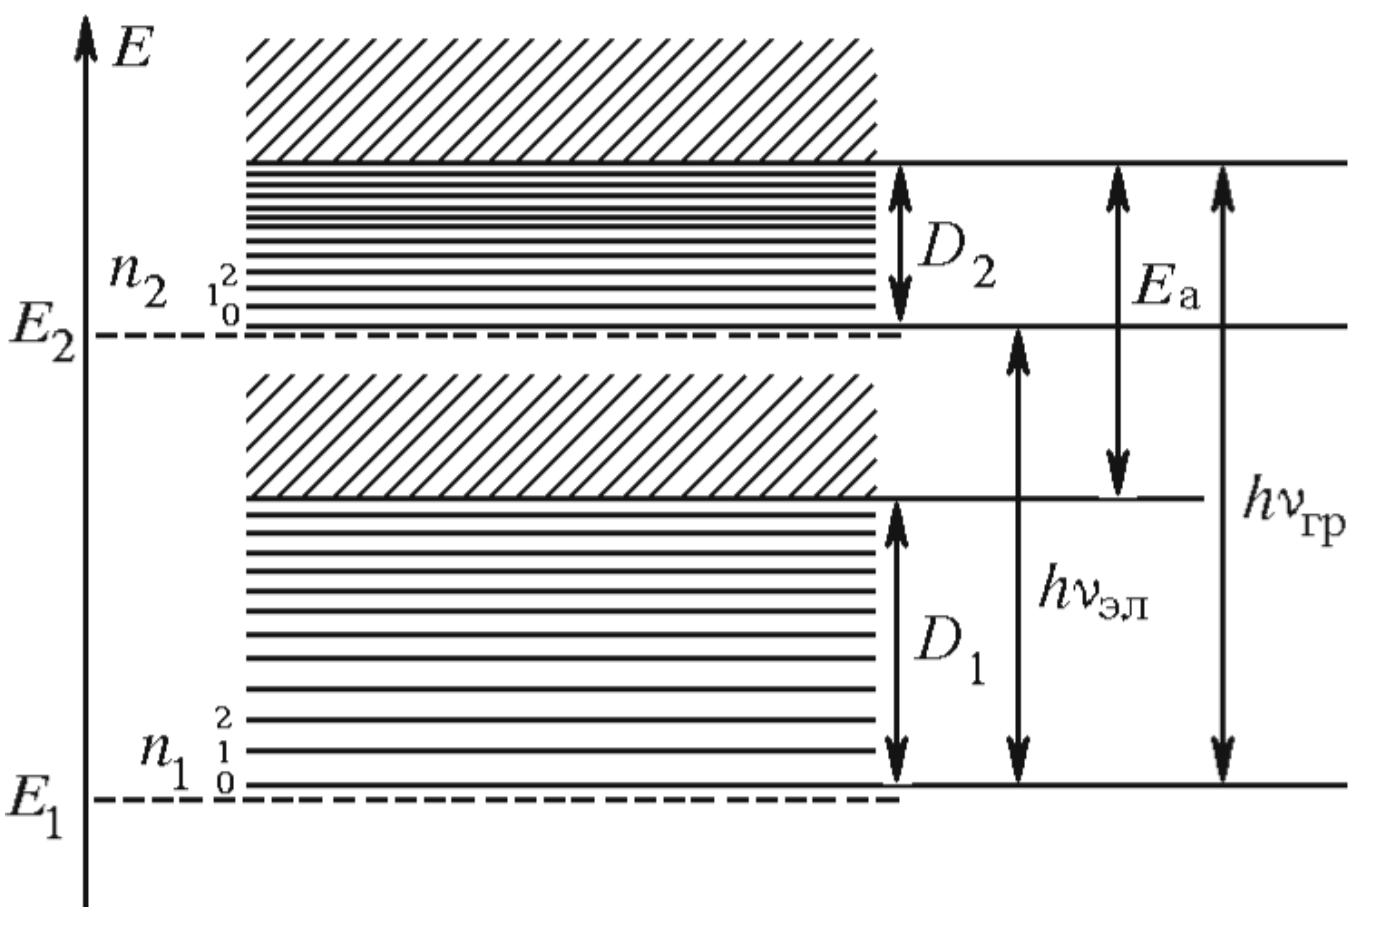
\includegraphics[scale = 0.3]{p4.png}
    \caption{Электронные и электронно-колебательные энергиетические уровни}
    \label{p4}
    \end{center}
\end{figure}

$E_A$ - энергия возбуждения атома возникающая при переходе молекулы из состояния 1 в область 
непрерывного спектра 2. \par
Энергия чисто электронного перехода $h\nu_{\text{эл}} = E_2 - E_1$\par
Граница схождения спектра, где происзодит переход молекулы в облатсь непрерывного спектра $h\nu_{\text{гр}}$\par

Все возможные линии поглощения для переходов между колебательными уровнями, налагающихся
на два соседних электронных состояния можно на серии , соответствующие одному и тому же
начальному состоянию. Эти серии называются сериями Деландра.


\begin{figure}[H]
    \begin{center}
    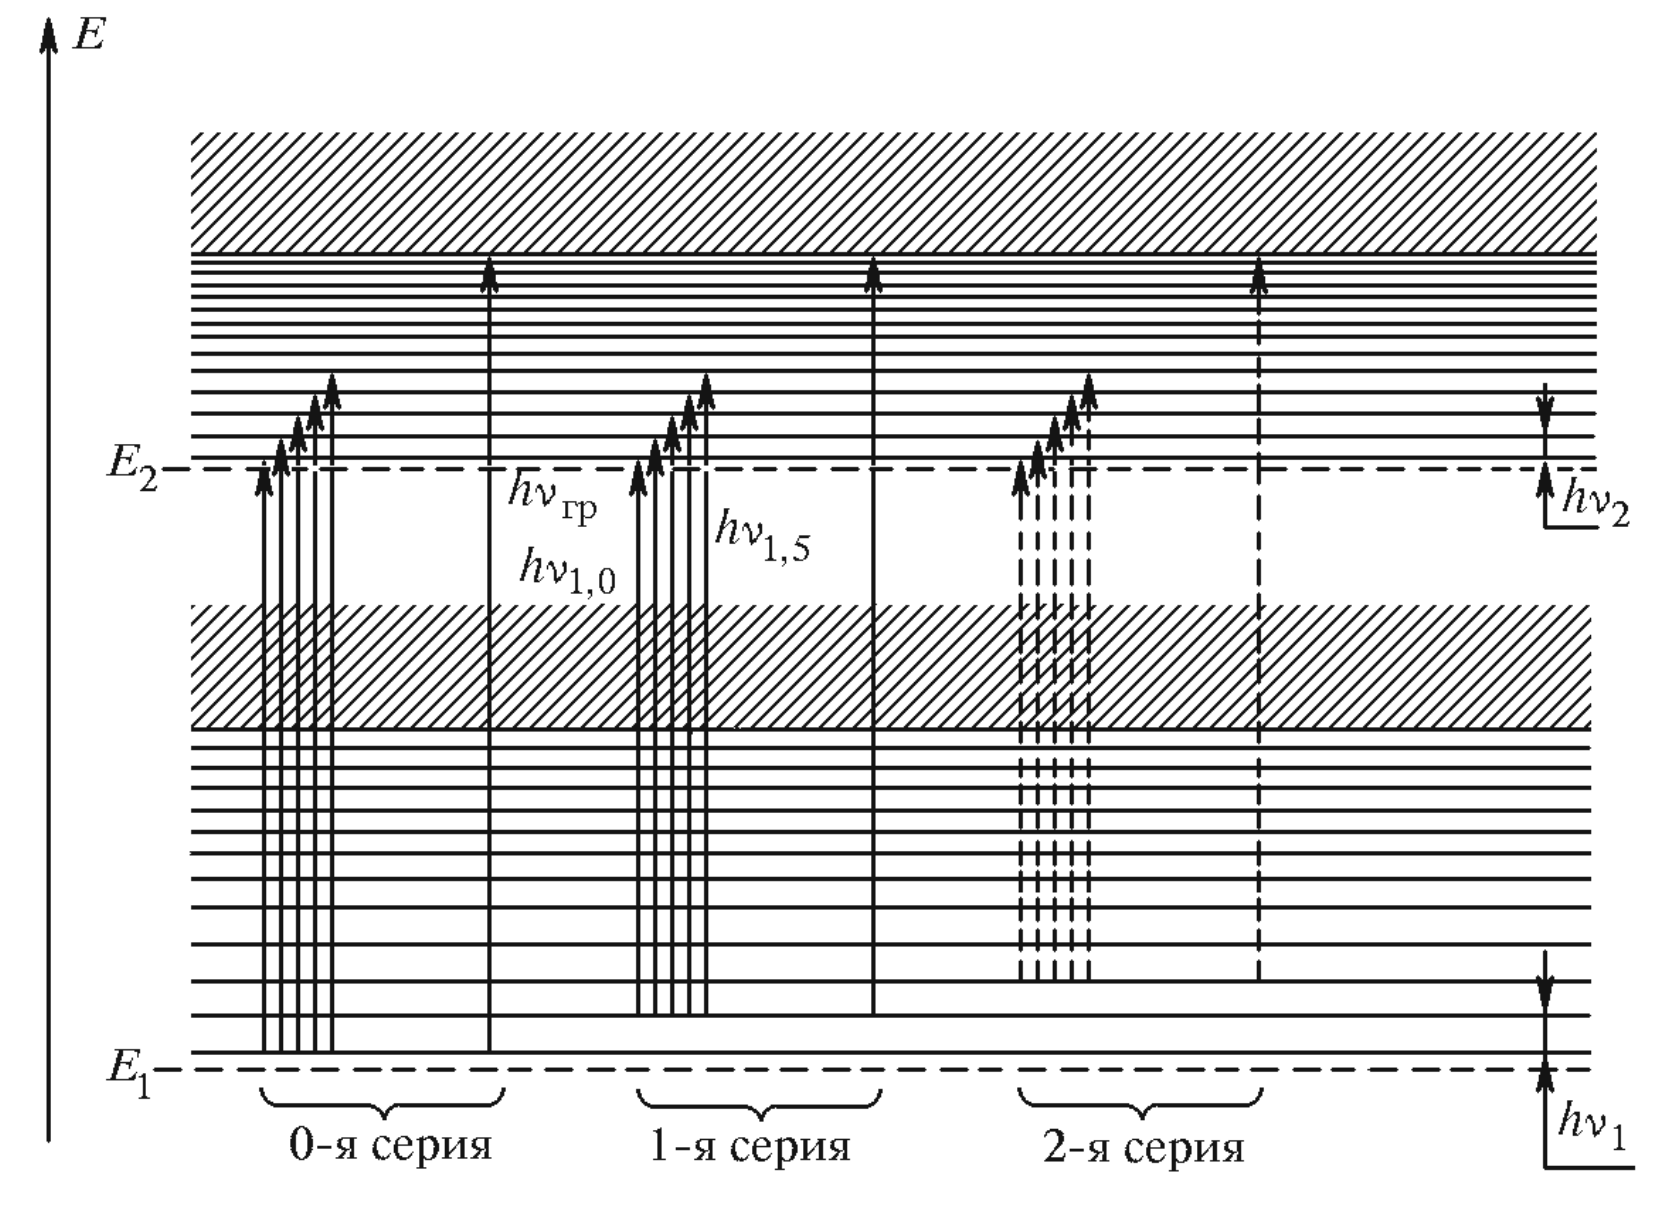
\includegraphics[scale = 0.3]{p5.png}
    \caption{Структура электронно-колебательного спеткра поглощения молекулы йода}
    \label{p5}
    \end{center}
\end{figure}

Для наблюдения таких серий необходимо достаточно много молекул в начальном состоянии.\par

Соотношения интенсивностей серий деландра пропорционально количеству молекул:
$$N_0 : N_1 : N_2 \approx 1 : 1/3 : 1/10$$

Энергетическое положение линий полгощения описывается выражением:
$$h\nu_{0,n_2} = (E_2 - E_1) + h\nu_2 (n_2+1/2) - 1/2 h\nu_1$$
Здесь пренебрегли ангармонизмом, для начальных серий можно пренебреч и энерг. расстояние между сериями:
$$h\nu_{0,n_2} - h\nu_{0,(n_2 - 1)} \approx h\nu_2$$
То есть равны колебательному кванту в возбужденном электронном состоянии.\par

Вся 1-я серия сдвинута в сторону меньших энергий на величину $h\nu_1$ на величину колебательного кванта основног состояния.

\begin{figure}[H]
    \begin{center}
    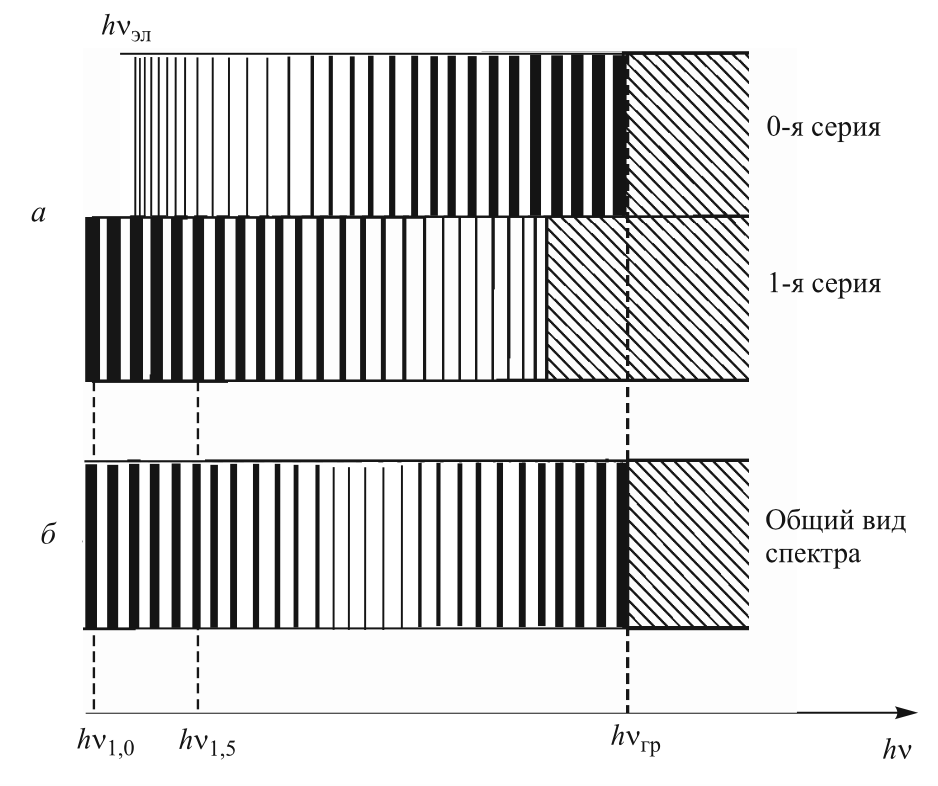
\includegraphics[scale = 0.38]{p6.png}
    \caption{Спектр поглощения паров йода}
    \label{p6}
    \end{center}
\end{figure}


\section{Экспериментальная установка}
Для измерения длин волн спектральных линий в работе используется стеклянно-призменный 
монохроматор-спектрометр УМ-2, предназначенный для спектральных исследований в диапазоне 
от 0,38 до 1 мкм

\begin{figure}[h]
	\begin{center}
	\begin{minipage}[h]{0.45\linewidth}
	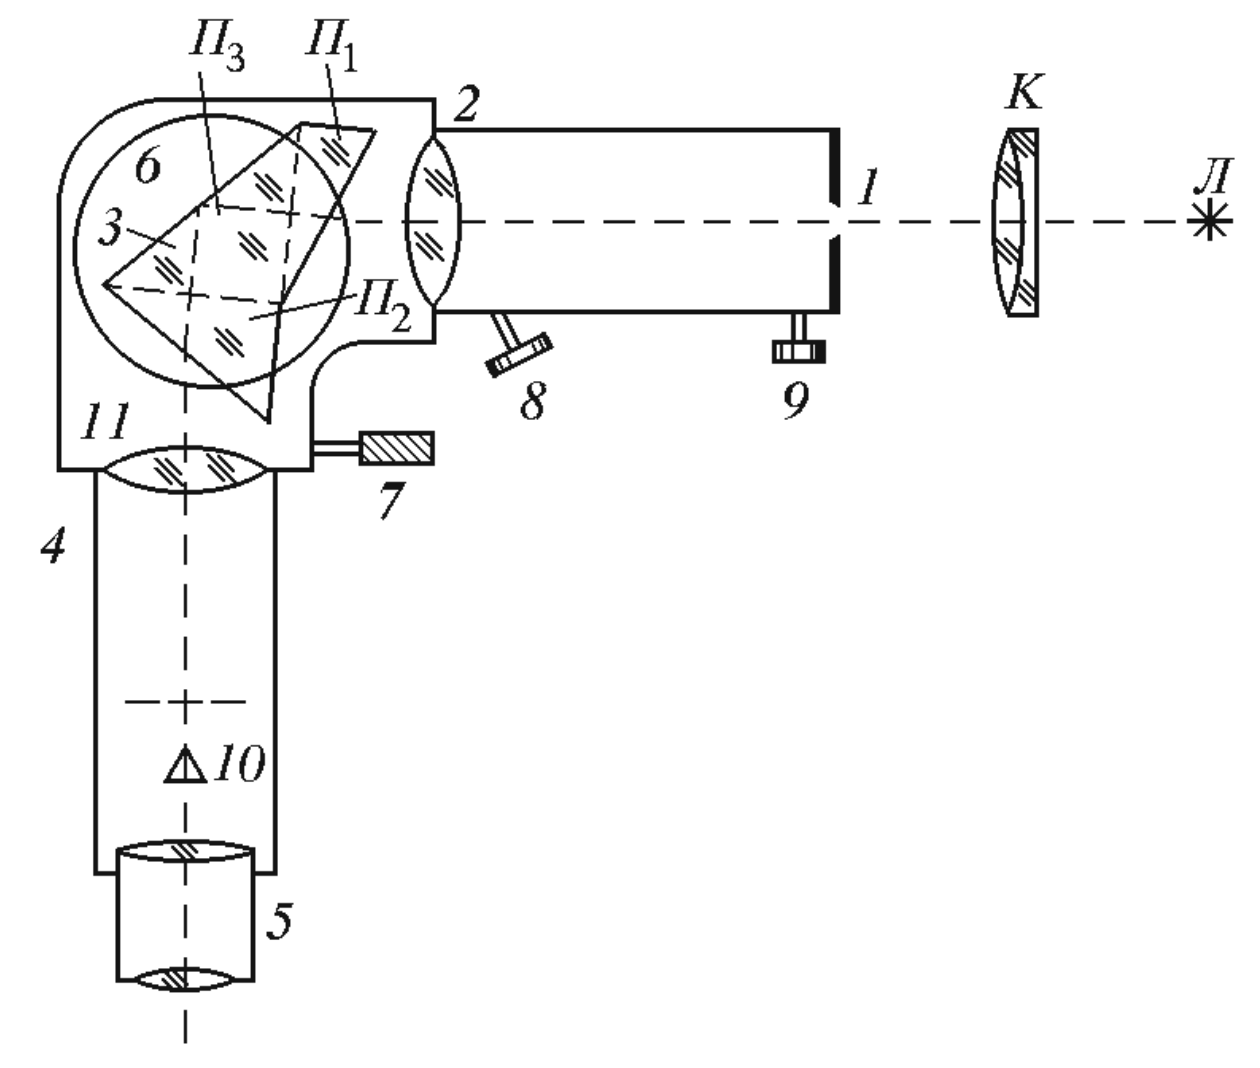
\includegraphics[width=1\linewidth]{p2.png}
	\caption{Установка для Водорода} 
	\label{p2}
	\end{minipage}
	\hfill 
	\begin{minipage}[h]{0.45\linewidth}
	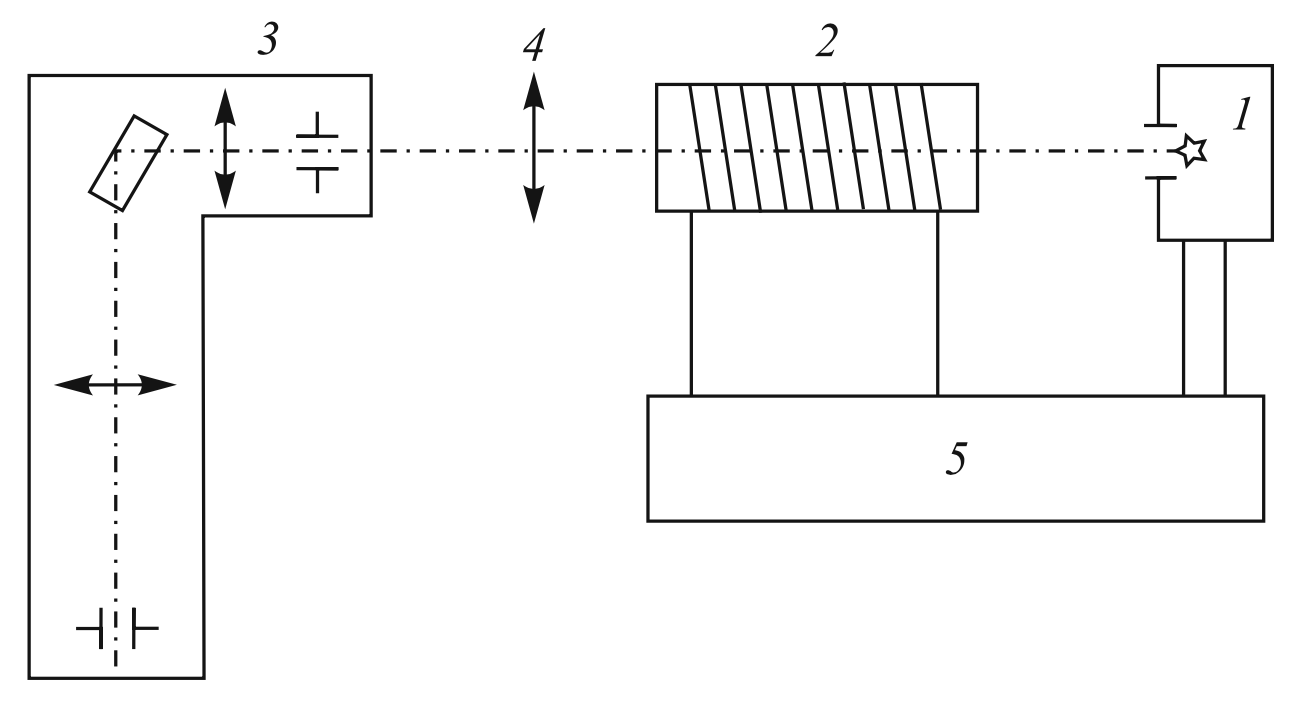
\includegraphics[width=1\linewidth]{p3.png}
	\caption{Установка для Йода}
	\label{p3}
	\end{minipage}
	\end{center}
\end{figure}

Спектрометр нуждается в дополнительной градуировке, проводящейся по спектрам неоновой и ртутной ламп с 
известными длинами волн спектральных линий.

\section{Выполнение работы}
\begin{enumerate}
    \item Выполним градуировку по неоновой и ртутной лампе:
    
    \begin{table}[H]
        \centering
        \begin{tabular}{|c|c|c|c|}
            \hline
            Neon $\lambda, \; \mathring{A}$ & Neon angle $^{\circ}$ &  Hg angle $^{\circ}$&Hg $\lambda, \; \mathring{A}$  \\
            \hline
            5401 & 2250 & 652 & 4047 \\ \hline
            5852 & 2512 & 1204 & 4358 \\\hline
            5882 & 2578 & 1870 & 4916 \\\hline
            5945 & 2558 & 2292 & 5461 \\\hline
            5976 & 2574 & 2470 & 5770 \\\hline
            6030 & 2598 & 2482 & 5791 \\\hline
            6074 & 2628 & 2686 & 6234 \\\hline
            6094 & 2638 & 2932 & 6907 \\\hline
            6143 & 2646 &  &  \\\hline
            6164 & 2656 &  &  \\\hline
            6217 & 2678 &  &  \\\hline
            6267 & 2698 &  &  \\\hline
            6305 & 2714 &  &  \\\hline
            6507 & 2790 &  &  \\\hline
        \end{tabular}
    \end{table}

    Сделаем фит полиномом 3й степени:

    \begin{figure}[H]
        \begin{center}
        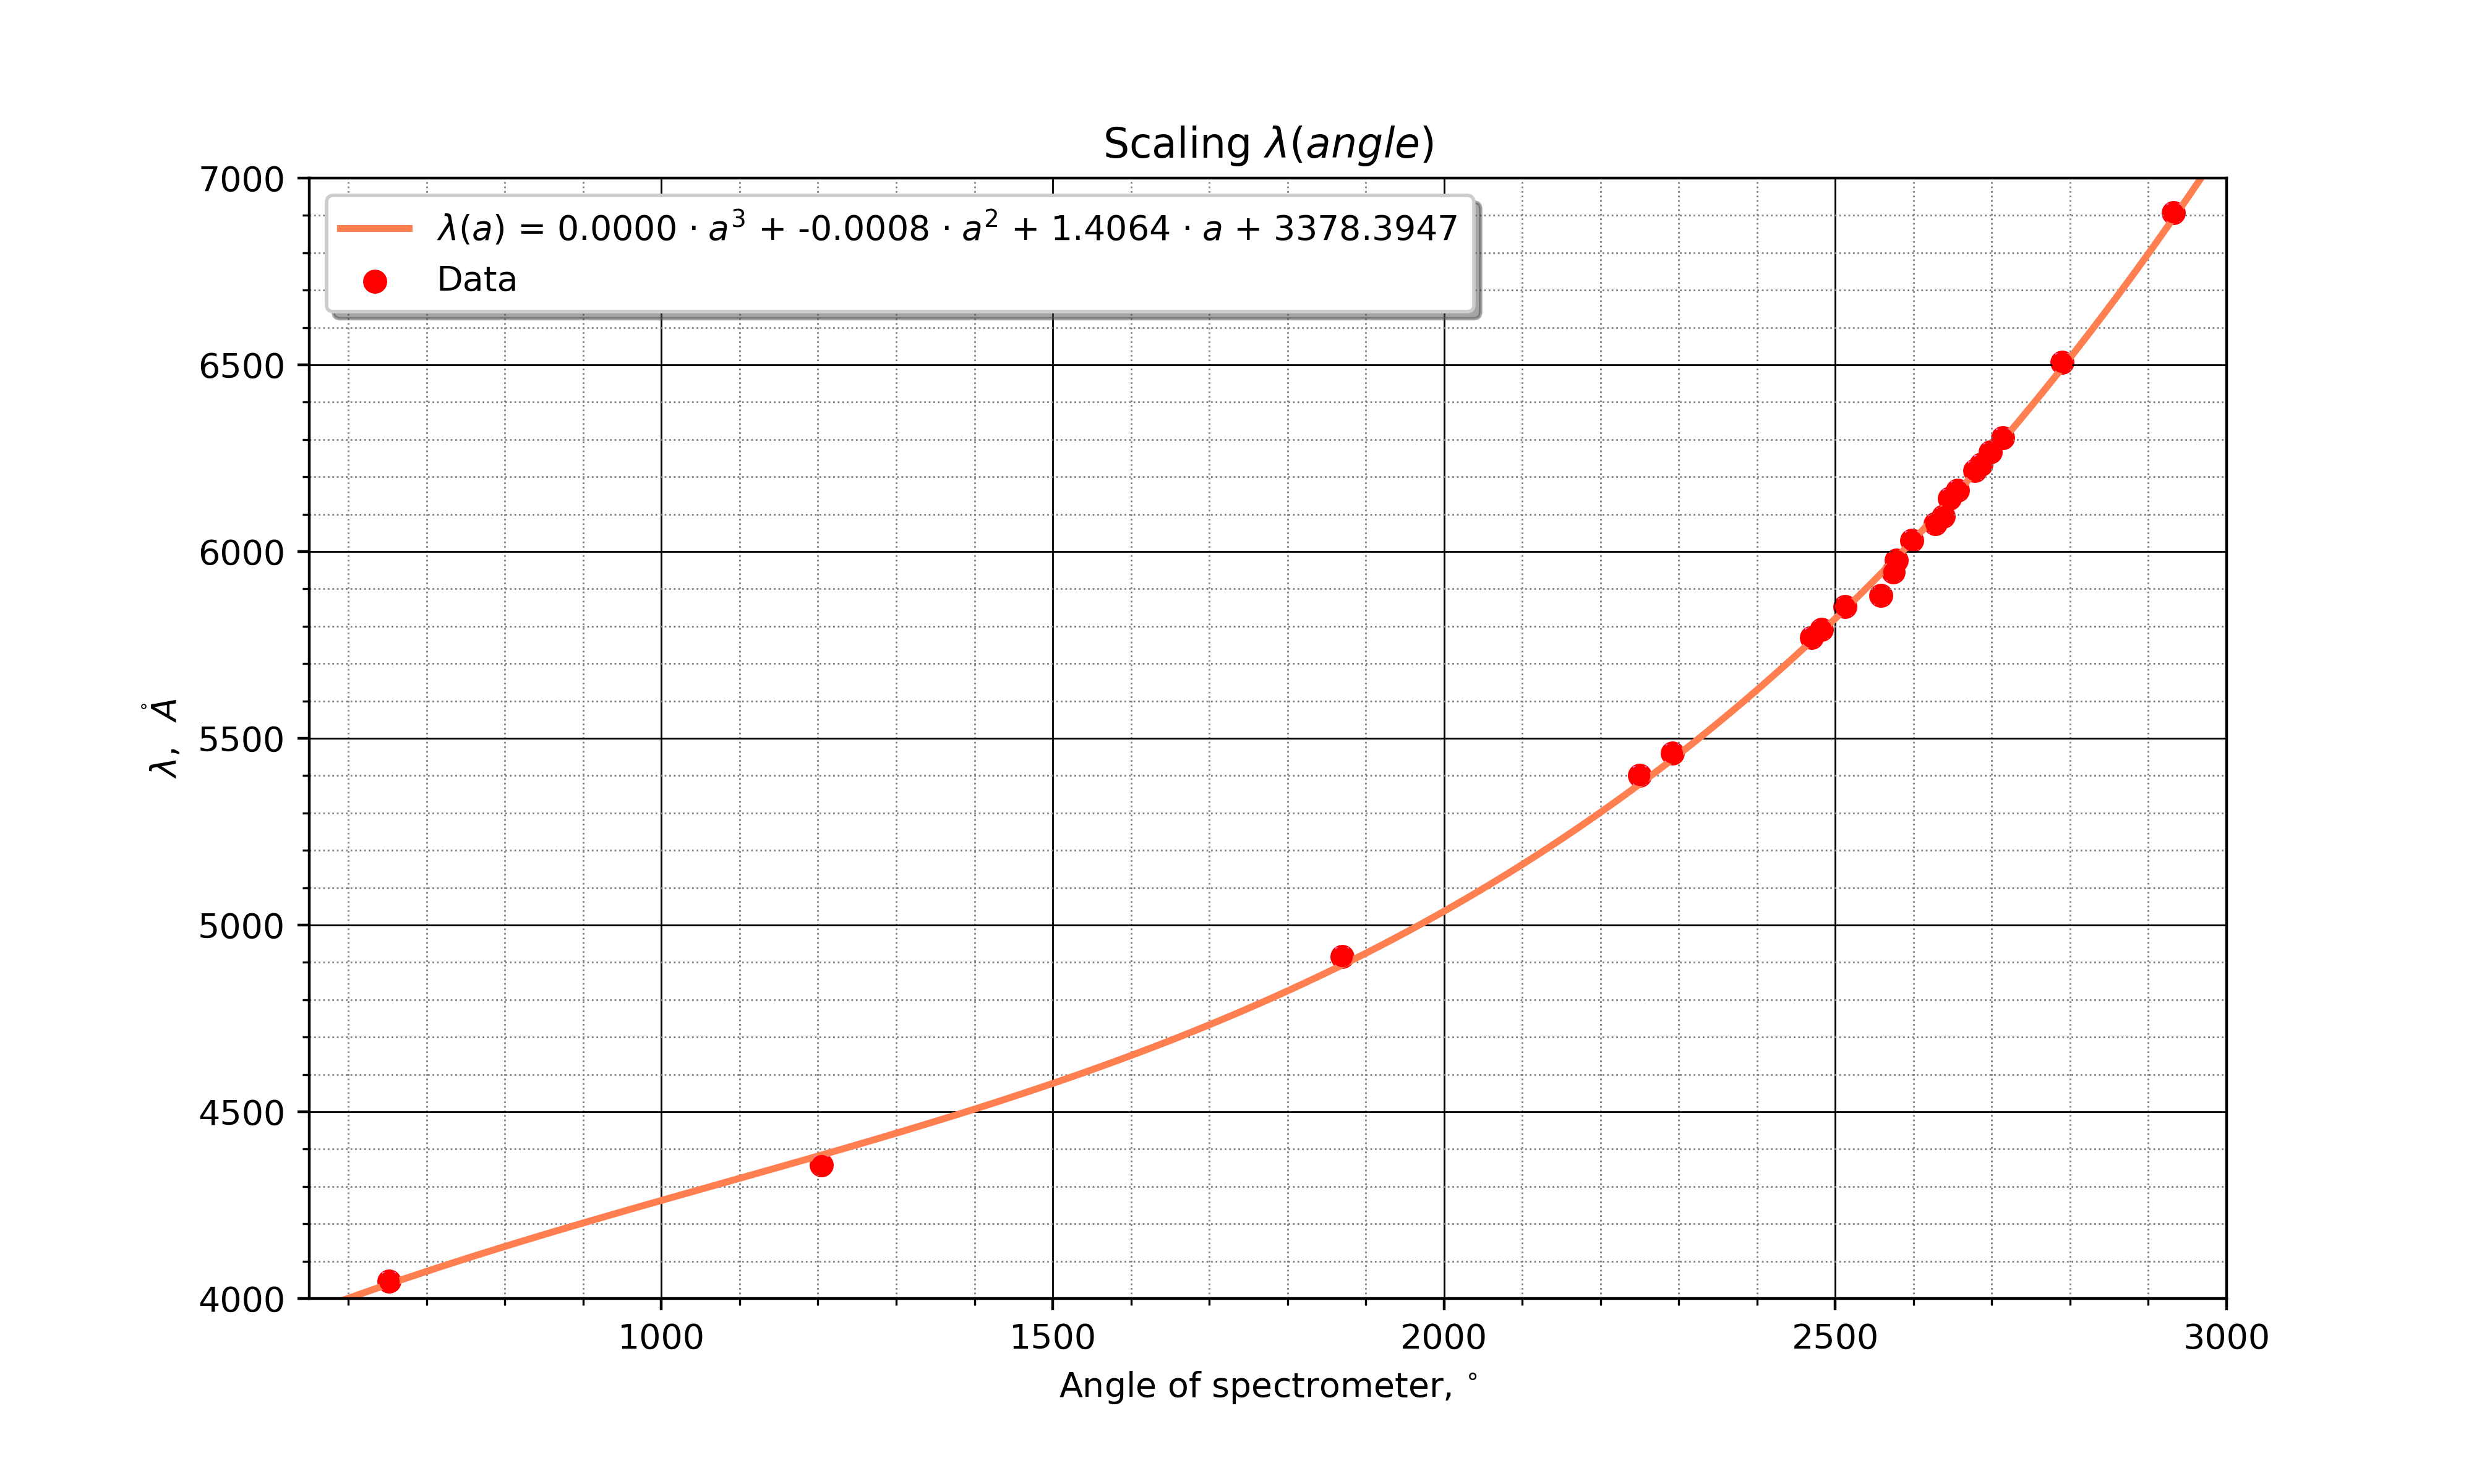
\includegraphics[scale = 0.6]{Scale.png}
        \caption{Градуировка по неону и ртути}
        \label{Neon}
        \end{center}
    \end{figure}

    Ошибка аппроксимации $\sim 19.4 \; \mathring{A}$

    \item По градуировочным графикам определим длины волн $H_{\alpha}, H_{\beta}, H_{\gamma}, H_{\delta}$

    \begin{table}[htb]
        \centering
        \begin{tabular}{|c|c|c|}
            \hline
            H line & H angle $^{\circ}$ &  $\lambda, \; \mathring{A}$  \\
            \hline 
            $H_{\alpha}$ & 2810 & 6545.5  \\\hline
            $H_{\beta}$ & 1814 & 4837.0  \\\hline
            $H_{\gamma}$& 1174 & 4365.8\\\hline
            $H_{\delta}$ & 740 & 4099.9 \\ \hline

        \end{tabular}
    \end{table}

    
    \item По формуле $\frac{1}{\lambda_{mn}} = RZ^2(\frac{1}{n^2} - \frac{1}{m^2})$ определим постоянные Ридберга:

    Усредним $R = 109772.9 \pm 715.5 cm^{-1} (\sim 0.7\%)$

    \item По градуировочной кривой определим длины волн поглащения йода\par
    $n_{1,0} - 2840^{\circ} - 6627.3 \; \mathring{A}$ - самая длиноволновая\par
    $n_{1,5} - 2772^{\circ} - 6444.9\; \mathring{A}$ - 6-я по счету слева\par
    $n_{\text{гр}} - 2026^{\circ} - 5068.1 \; \mathring{A}$ - граница схождения спектра\par
    \item Вычислим в электронвольтах энергию колебательного кванта возбужденного состояния молекулы йода:\par
    $h\nu_2 = (h\nu_{1,5} - h\nu_{1,0})/5 = 0.0106$ (эВ)
    \item Используя $h\nu_1 = 0.027$(эВ) и энергию возбуждения атома $E_A = 0.94$(эВ) $h\nu_{\text{гр}} \approx 2.45$(эВ)  $h\nu_{1,0} \approx 1.93$(эВ) вычислим:
    \begin{itemize}
        \item Энергию электронного перехода $h\nu_{\text{эл}} = h\nu_{1,0} + h\nu_1 \approx 1.95$ (эВ)
        \item Энергия диссоциации из основного состояния $D_1 = h\nu_{\text{гр}} - E_A \approx 1.51$ (эВ)
        \item Энергия диссоциации из возбужденного состояния $D_2 = h\nu_{\text{гр}} - h\nu_{\text{эл}} \approx 0.5$ (эВ)
    \end{itemize}
     
\end{enumerate}

\section{Вывод}
В данной работе исследованы сериальные закономерности в оптических спектрах водорода и йода. 
Вычислена постоянная Ридберга для водорода по результатам измерения. Вычислена энергия колебательного 
кванта молекулы йода и энергия диссоциации в основном и возбужденном состояниях.

\end{document}